\section{Teoremas de existencia y unicidad de las soluciones}

La clase de las ecuaciones diferenciales ordinarias que son integrables por cuadraturas es muy limitada, por ello la mayor\'ia de las ecuaciones se resuelve usando m\'etodos de aproximaci\'on num\'erica.


\begin{teorema}
Si en la ecuaci\'on
$$
\dfrac{\mathrm{d}f}{\mathrm{d}t}=f(x,y)
$$
la funci\'on
$f$ es continua en $D=\left[x_0-a,x_0+a\right]\times\left[y_0-b,y_0+b\right]$, adem\'as $f$ es Lipschitz-continua en $D$, es decir que existe una constante $N$ tal que $|f(x_1,y_1)-f(x_2,y_2)|\leq N|y_1,y_2|$ para $(x_i,y_i)\in D$.

Entonces existe una soluci\'on \'unica $y=\bar{y}(x)$ en el intervalo $\left[x_0-H,x_0+H\right]$ que satisface $y(x_0)=y_0$ y donde $H<\min\{a,\frac{b}{M},\frac{1}{N}\}$, $M=\max_{D}\{|f(x,y)|\} $
\end{teorema}


Las condiciones del teorema  requieren aclaraci\'on. La soluci\'on para la ecuaci\'on, que satisface las condiciones iniciales  existe s\'olo para $x\in [x_0-a,x_0+a]$ pero $y$ puede existir fuera del rect\'angulo $D$. Es decir $y=y_0\pm b$ para alg\'un $x=x_1\in[x_0-a,x_0+a]$. Si $x_1>x_0$ para $x>x_1$, la soluci\'on puede no estar definida.

Podemos garantizar que $y=\bar{y}(x)$ no se sale de $D$ cuando $x\in[x_0-H,x_0+H]$ con $H<a$ y $H<\frac{b}{M}$, $M=\tan\alpha$. Donde $\alpha$ es el coeficiente angular de latangente a la curva integral buscada. Si estas rectas se salen de $D$ entonces las absisas de los puntos de corte son $x_0\pm\dfrac{b}{M}$. As\'i la absisa  del punto de salida de lacurva inegral de $D$ puede solamen
te ser menor o igual que $x_0+\frac{b}{M}$ y mayor o igual que $x_0-\frac{b}{M}$. Puede mostrarse la existencia  dela soluci\'on en $[x_0-H,x_0+H]$ con $H=\min\{a,\frac{b}{M}\}$ pero ser\'a m\'as sencillo mostrarlo para $H<\min\{a,\frac{b}{M},\frac{1}{N}\}$

\begin{figure}[H]
\centering
\begin{tikzpicture}
\draw[](-0.3,0)--(6,0);
\draw (1,5)--(5,5);
\draw (1,5)--(1,2);
\draw (5,2)--(5,5);
\draw (1,2)--(5,2);
\draw[](0,-0.3)--(0,6);
\draw (1.3,2)to[bend left](3.5,3.5);
\filldraw (3.5,3.5) circle (2pt) ;
\draw (3.5,3.5)to[bend right](4.8,5);
\draw[dotted](3.5,3.5)--(3.5,0) node[pos=1.14]{$x_0$};
\draw[dotted](3.5,3.5)--(0,3.5) node[pos=1.1]{$y_0$};
\draw[dotted](1,5)--(1,0) node[pos=1.1]{$x_0-a$};
\draw[dotted](5,2)--(5,0) node[pos=1.2]{$x_0+a$};
\draw[dotted](1,5)--(0,5) node[pos=1.5]{$y_0+a$};
\draw[dotted](5,2)--(0,2) node[pos=1.1]{$y_0-a$};
\end{tikzpicture}
    \caption{}
    \label{fig:my_label}
\end{figure}

\begin{figure}[H]
    \centering
    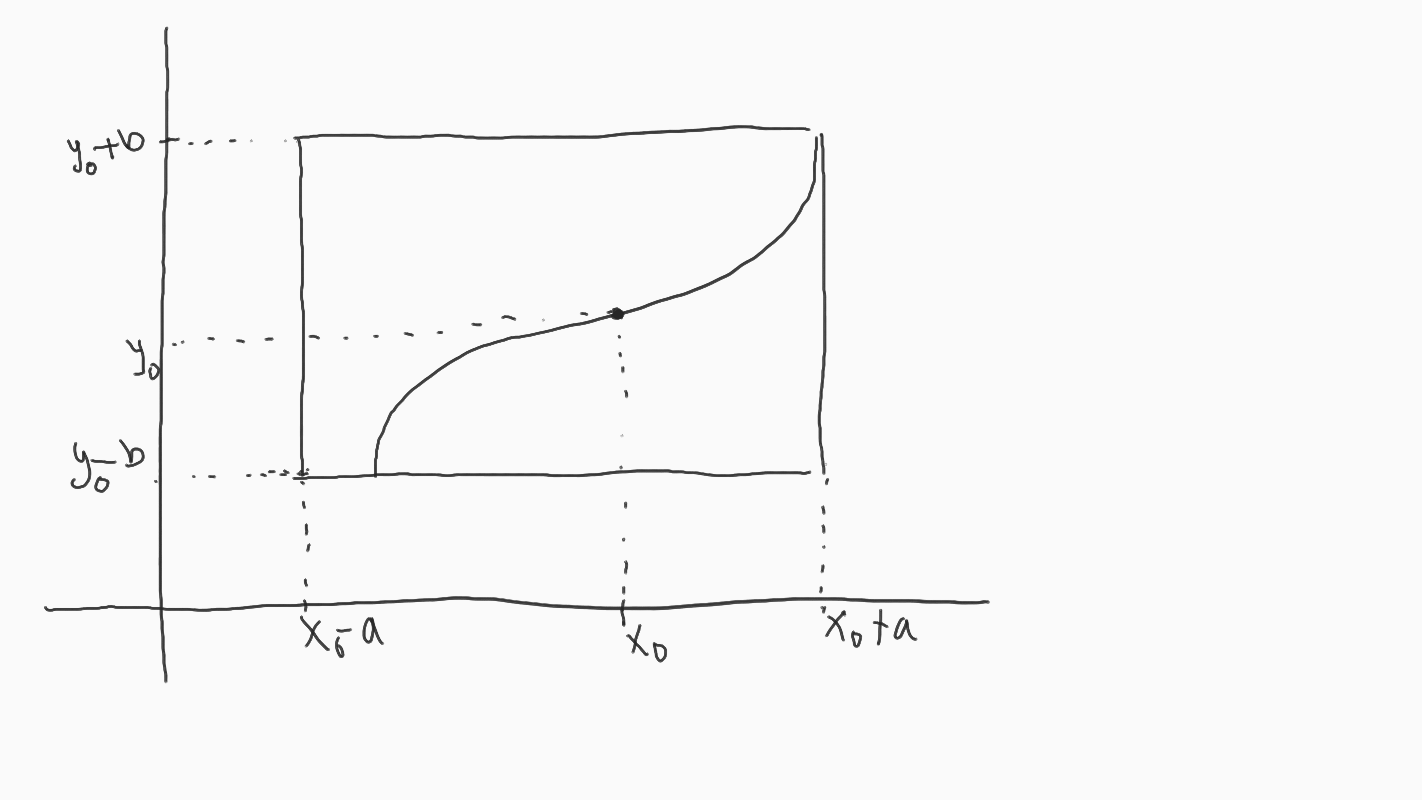
\includegraphics[scale=0.25]{graficas1.png}
    \caption{Caption}
    \label{fig:my_label}
\end{figure}


La condici\'on de Lipschitz 
$$
|f(x_1,y_1)-f(x_2,y_2)|\leq N(y_1-y_2)
$$
puede ser sustituida por otra m\'as fuerte, pero m\'as f\'acilmente comprobable, la existencia de $\partial_{y} f^{'}$ en $D$ y que sea acotada.

En efecto para $(x,y)\in D$ y $|f'_y(x,y)|\leq N$ entonces por el teorema del valor intermedio:
$$
|f(x_1,y_1)-f(x_2,y_2)|=|f'_y(x,\xi)|-|y_1-y_2| 
$$
con $\xi\in (y_1,y_2)$. As\'i $(x,\xi)\in D$ y $|f_y(x,\xi)|\leq N$ , $|f(x,y_1)-f(x,y_2)|\leq N|y_1-y_2|$.

\begin{proof}
Observemos primero que 
$$
\left.\begin{array}{cc}
    \dfrac{\mathrm{d}y}{\mathrm{d}x}&=f(x,y)  \\
    &\\
    y(x_0) &=y_0 
\end{array}\right.
$$
es equivalente a
$$
y=y_0+\int_{x_0}^xf(x,y)\mathrm{d}x
$$

En efecto:
$$
\int_{x_0}^x\frac{\mathrm{d}y}{\mathrm{d}x}\mathrm{d}x=\int_{x_0}^xf(x,y)\mathrm{d}x
$$
así
$$
y(x)-y(x_0)=\int_{x_0}^xf(x,y)\mathrm{d}x
$$
y por tanto
$$
y(x)=y_0+\int_{x_0}^xf(x,y)\mathrm{d}x
$$
Ahora, hagamos una aproximaci\'on de  la soluci\'on usando Euler
$$
y=y_n(x)
$$
con paso $h_n=\frac{H}{n}$ en $[x_0,x_0+H]$.

La poligonal asociada a la aproximaci\'on de Euler no sale de la regi\'on $D$ pues el coeficiente angular de cada segnmento es menor  que $M$ en m\'odulo.

A continuaci\'on probaremos que
\begin{enumerate}
\item la sucesi\'on  $(y_n)$ converge uniformemente.
\item $\bar{y}(x)=\lim_{n\rightarrow infty}y_n$ es soluci\'on para la ecuaci\'on integral.
  \item La soluci\'on es \'unica
\end{enumerate} 

Probemos $\bf{(1)}$. En efecto $y'_n(x)=f(x_k,y_k)$ 
\end{proof}
 